\noindent Myonen, Elektronen und Tauonen bilden zusammen mit ihren jeweiligen
Neutrinos im Standardmodell der Elementarteilchen die Familie der Leptonen. Alle
genannten Teilchen besitzen einen halbzahligen Spin. Das Myon, das Elektron
sowie das Tauon tragen zusätzlich die Elementarladung, während ihre Neutrinos
ungeladen sind.
\begin{figure}
  \centering
  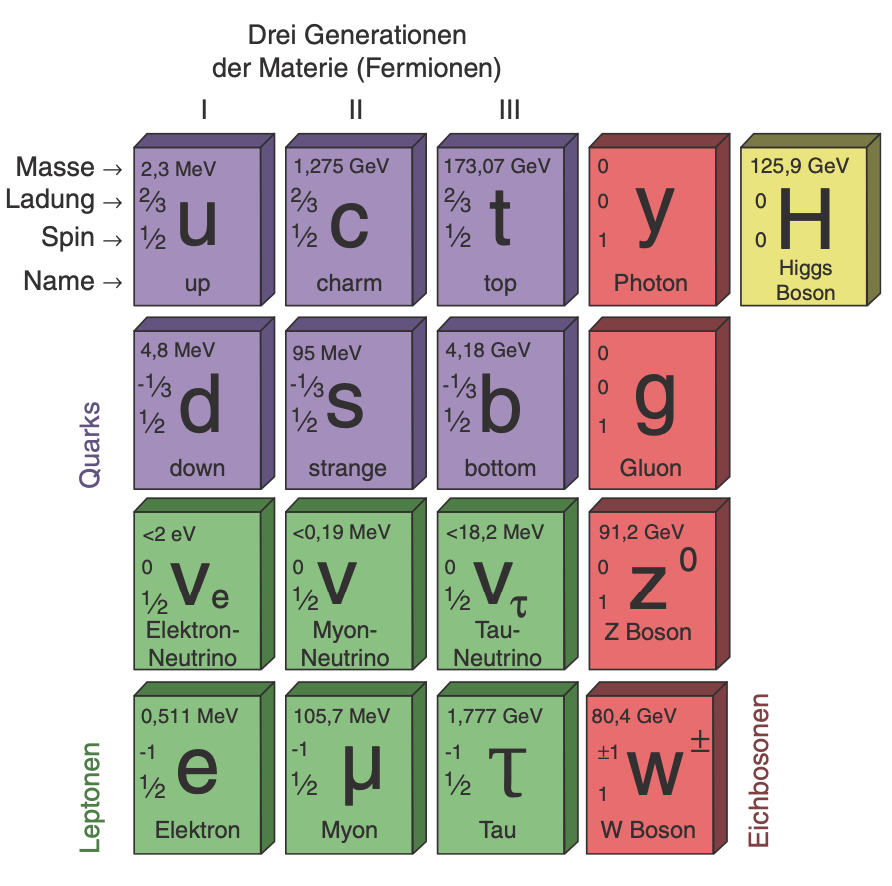
\includegraphics[scale=0.5]{resources/standardmodell.png}
  \caption{Fermionische Elementarteilchenfamilien mit ihren zugehörigen
  Wechselwirkungsbosonen und dem Higgs-Boson \cite{großforschung}.}
  \label{fig:01}
\end{figure}
\noindent Beim Zerfall geladener Pionen $\pi^{\pm}$ in den oberen Schichten
der Erdatmosphäre in einer Höhe von etwa $\SI{15}{\kilo\meter}$ entstehen
geladene Myonen gemäß den Zerfallsgleichungen \ref{eqn:01} \cite{grupen}.
\begin{align}
  \ce{\symup{\pi}+ -> \symup{\mu}+ + \symup{\nu}}, \qquad
  \ce{\symup{\pi}- -> \symup{\mu}- + \bar{\symup{\nu}}}.
  \label{eqn:01}
\end{align}
\noindent Die entstehenden Myonen sind allerdings nicht stabil und zerfallen
unter der schwachen Wechselwirkung
mit einer mittleren Lebensdauer von etwa $\tau = \SI{2.2}{\micro\second}$ in
ein Elektron und ein Elektron-Antineutrino (für $\ce{\symup{\mu}- }$) bzw.
ein Positron und ein Elektron-Neutrino (für $\ce{\symup{\mu}+ }$) mitsamt ihrer
jeweiligen Myon-Antineutrinos bzw. Myon-Neutrinos, ohne dabei die
Leptonenzahlerhaltung zu verletzen \cite{grupen}. \\
\newline
\noindent Eine klassische Betrachtung der möglichen freien Weglänge der Myonen
bis zu ihrem Zerfall zeigt schnell, dass diese selbst unter der Annahme, dass
sie sich mit Lichtgeschwindigkeit fortbewegen, maximal eine Strecke von zirka
$s_0 = \SI{660}{\meter}$ zurücklegen können. Der scheinbare Widerspruch, dass Myonen
auf der Erdoberfläche detektiert werden können löst sich erst unter
Berücksichtigung relativistischer Effekte. So beträgt die zurückgelegte Strecke
im Ruhesystem der Myonen aufgrund der Längenkontraktion unter der Annahme einer
mittleren Geschwindigkeit der Myonen von $\bar{v}_\text{Myon} = 0.9999 \cdot c$
etwa
\begin{align}
s =\frac{1}{\sqrt{\left(1 - \frac{{v_\text{Myon}}^2}{c^2} \right)}} \cdot s_0 \approx \SI{46.7}{\kilo\meter}.
\label{eqn:02}
\end{align}
